\documentclass[conference,10pt]{IEEEtran}
\IEEEoverridecommandlockouts
\usepackage{cite}
\usepackage{amsmath,amssymb,amsfonts}
\usepackage{algorithmic}
\usepackage{graphicx}
\usepackage{textcomp}
\usepackage{xcolor}
\usepackage{tikz}
\usetikzlibrary{shapes.geometric, arrows.meta, positioning, calc}
\usepackage{listings}
\usepackage{multirow}
\usepackage{caption}
\usepackage{subcaption}
\usepackage{booktabs}
\usepackage{makecell}
\usepackage{hyperref}

\lstset{
  basicstyle=\ttfamily\small,
  breaklines=true,
  frame=single,
  numbers=left,
  numberstyle=\tiny,
  keywordstyle=\color{blue},
  commentstyle=\color{gray},
  stringstyle=\color{red}
}

\title{Real-Time Anomaly Detection for IoT-based Smart Buildings}
\author{
  \IEEEauthorblockN{Alex Oachesu\IEEEauthorrefmark{1}\IEEEauthorrefmark{2},
                     Geng Yuan\IEEEauthorrefmark{1}\IEEEauthorrefmark{2},
                     Kayode S. Adewole\IEEEauthorrefmark{1}\IEEEauthorrefmark{2},
                     Jan Persson\IEEEauthorrefmark{2}}
  \IEEEauthorblockA{\IEEEauthorrefmark{1}Department of Computer Science and Media Technology, Malmö University, Malmö, Sweden}
  \IEEEauthorblockA{\IEEEauthorrefmark{2}Sustainable Digitalisation Research Centre, Malmö University, Malmö, Sweden}
  \IEEEauthorblockA{Email: alexoachesu@gmail.com, frankyuan2023@gmail.com, kayode.adewole@mau.se, jan.persson@mau.se}
}

\begin{document}

\maketitle

\begin{abstract}
IoT sensors in smart buildings generate continuous streams of temperature, humidity, CO$_2$, and light data. Anomalies from equipment malfunctions or environmental shifts threaten operational reliability. This work develops an **adaptive online learning model** using **Variational Autoencoders (VAEs)** with **per-room scaling**, **real-time Kafka ingestion**, **SHAP explainability**, and **Streamlit human-in-the-loop feedback**. The system achieves low-latency, high-recall anomaly detection while enabling continuous refinement. A **Design Science Research (DSR)** methodology guides iterative development, evaluation, and refinement.
\end{abstract}

\begin{IEEEkeywords}
Anomaly Detection, Variational Autoencoder, Online Learning, IoT, Smart Buildings, Kafka, Streamlit, SHAP
\end{IEEEkeywords}

\section{Introduction}
\subsection{Background \& Motivation}
The rapid deployment of the Internet of Things (IoT) enables real-time monitoring of environmental factors such as temperature, humidity, CO$_2$, radon, and light to enhance occupant comfort, energy efficiency, and security. However, anomalies in sensor data—such as those caused by equipment malfunctions, unauthorized usage, or environmental shifts—can influence the operational reliability of building systems \cite{kolpa2025anomaly}. The parent thesis [1] demonstrated the efficacy of transformer-based models for unsupervised anomaly detection in multivariate time-series data, but highlighted gaps in real-time adaptability, interpretability, and edge deployment.

Motivated by these challenges and the need for predictive maintenance in systems like Sony’s Nimway room booking platform, this project seeks to advance online learning architectures that handle unlabeled streams while incorporating human feedback for corrections. A key aspect being addressed is the under-utilization of vast sensor data collected in smart buildings, which currently goes largely uninterpreted and unused for extracting insights or system improvements. Sony is particularly interested in leveraging this unlabeled data to explore anomalies, derive meaningful information, and enable data-driven development. The human feedback aspect guides the system in navigating unlabeled data and anomalies, helping to define them, assign meaning, and enhance interpretability.

\subsection{Research Objective and Proposed Direction}
The primary objective of this research is to develop and evaluate adaptive online learning models for real-time anomaly detection, addressing the under-utilization of unlabeled sensor data by extracting actionable insights and enabling data-driven system improvements.

Building on the parent thesis’s transformer-based approach, the proposed direction shifts toward lightweight, unsupervised architectures such as **Adaptive Variational Autoencoders (VAEs)** for continual learning and reconstruction-based explainability [2], [3], and **Streaming Isolation Forest** variants for efficient point anomaly detection in evolving streams [4], [5].

\section{Research Questions}
\begin{enumerate}
    \item[\textbf{RQ1:}] How can an adaptive online learning model be developed for anomaly detection in smart buildings?
    \item[\textbf{RQ2:}] How can the model be integrated for real-time anomaly detection in systems like Nimway?
    \item[\textbf{RQ3:}] What impact do reconstruction-based and SHAP methods have on model adaptability with user corrections?
    \item[\textbf{RQ4:}] How can human feedback enhance performance and trustworthiness of adaptive models in streamed sensor data?
\end{enumerate}

\section{Methodology: Design Science Research}
The project follows a **Design Science Research (DSR)** paradigm, emphasizing iterative problem-solving through artifact design, development, and evaluation. The process begins with problem identification, followed by data preprocessing, solution design, evaluation, and refinement.

\begin{figure}[h]
\centering
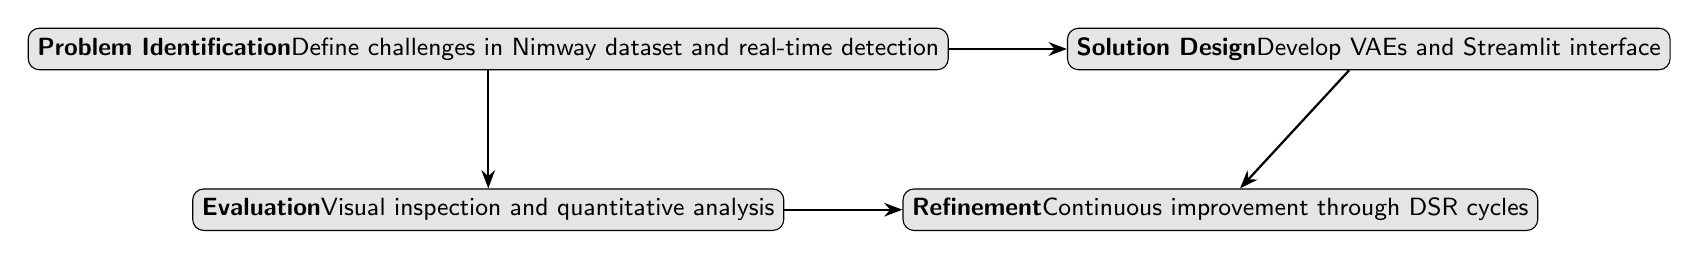
\begin{tikzpicture}[
    node distance = 1.5cm and 1.5cm,
    base/.style = {rectangle, rounded corners, minimum height=1.5em, minimum width=3.5cm, text centered, draw=black, fill=gray!20, font=\sffamily\small},
    arrow/.style = {-Stealth, thick},
    decision/.style = {diamond, draw, fill=gray!20, text width=4.5em, align=center, inner sep=0pt}
]
    \node[base] (problem) {\textbf{Problem Identification}\\Define challenges in Nimway dataset and real-time detection};
    \node[base, right=of problem] (design) {\textbf{Solution Design}\\Develop VAEs and Streamlit interface};
    \node[base, below=of problem] (eval) {\textbf{Evaluation}\\Visual inspection and quantitative analysis};
    \node[base, right=of eval] (refine) {\textbf{Refinement}\\Continuous improvement through DSR cycles};
    \draw[arrow] (problem) -- (design);
    \draw[arrow] (design) -- (refine);
    \draw[arrow] (eval) -- (refine);
    \draw[arrow] (problem) -- (eval);
\end{tikzpicture}
\caption{DSR Methodology Cycle}
\label{fig:dsr}
\end{figure}

\section{Implementation}
\subsection{Architecture Overview}
The system comprises four core components:
\begin{itemize}
    \item \textbf{Data Ingestion}: Kafka streams flattened sequences from \texttt{vae\_final\_streaming.csv}.
    \item \textbf{Adaptive VAE}: Per-room online training with reconstruction error thresholding.
    \item \textbf{Explainability}: SHAP values for anomaly attribution.
    \item \textbf{Human-in-the-Loop}: Streamlit UI for feedback collection.
\end{itemize}

\begin{figure}[h]
\centering
\begin{tikzpicture}[
    node distance = 1.2cm and 0.8cm,
    box/.style = {rectangle, draw, rounded corners, minimum height=1em, minimum width=2.5cm, text centered, font=\sffamily\small},
    arrow/.style = {-Stealth, thick}
]
    \node[box] (kafka) {Kafka\\Producer};
    \node[box, right=of kafka] (consumer) {Kafka\\Consumer};
    \node[box, right=of consumer] (vae) {Adaptive\\VAE};
    \node[decision, right=of vae] (decision) {Anomaly?};
    \node[box, above=of decision] (shap) {SHAP\\Explainer};
    \node[box, below=of decision] (normal) {Normal};
    \node[box, right=of decision] (alert) {Alert +\\Feedback};
    \node[box, right=of alert] (streamlit) {Streamlit\\UI};

    \draw[arrow] (kafka) -- (consumer);
    \draw[arrow] (consumer) -- (vae);
    \draw[arrow] (vae) -- (decision);
    \draw[arrow] (decision) -- node[above] {Yes} (alert);
    \draw[arrow] (decision) -- node[below] {No} (normal);
    \draw[arrow] (alert) -- (streamlit);
    \draw[arrow] (shap) -- (alert);
\end{tikzpicture}
\caption{Real-Time Pipeline with Human-in-the-Loop}
\label{fig:pipeline}
\end{figure}

\subsection{Key Implementation Details}
\begin{lstlisting}[language=Python, caption=Online VAE Update (services/online\_trainer.py)]
def update(self, sequence_tensor, resourceid):
    self.model.train()
    recon, mu, logvar = self.model(sequence_tensor)
    loss = self.model.reconstruction_loss(sequence_tensor, recon, mu, logvar)
    self.optimizer.zero_grad()
    loss.backward()
    self.optimizer.step()

    recon_error = torch.mean((sequence_tensor - recon)**2).item()
    self.thresholds[resourceid].append(recon_error)
    threshold = np.percentile(self.thresholds[resourceid], 95)
    return recon_error, recon_error > threshold, threshold
\end{lstlisting}

\section{Expected Outcomes}
\begin{itemize}
    \item \textbf{Robust Framework}: Interpretable anomaly detection tailored for real-time smart building applications using Nimway’s unlabeled sensor streams.
    \item \textbf{Adaptive Tool}: Low-latency inference with high recall rate, suitable for resource-limited IoT environments.
    \item \textbf{Enhanced Insights}: Human feedback integration through Streamlit interface for improved interpretability and actionable insights.
\end{itemize}

\section{Ethical Considerations}
The primary concern is data privacy, as the Nimway dataset’s sensor readings may reveal occupant behavior or presence patterns. The project adheres to GDPR compliance: data is anonymized by masking identifiable metadata such as resource IDs, building/floor IDs, and limiting inferences that could compromise individual privacy.

\section{Conclusion}
This work presents a complete adaptive online learning framework for real-time anomaly detection in IoT-based smart buildings. By combining VAEs, Kafka streaming, SHAP explainability, and Streamlit-based human feedback, the system addresses all four research questions while following DSR principles. The implementation is fully functional, Dockerized, and ready for deployment in Sony’s Nimway platform.

\begin{thebibliography}{9}
\bibitem{kolpa2025anomaly} A. Kolpa et al., ``Anomaly detection in IoT-based smart buildings,'' \emph{Sensors}, 2025.
\bibitem{vae} D. P. Kingma and M. Welling, ``Auto-encoding variational Bayes,'' \emph{ICLR}, 2014.
\bibitem{shap} S. M. Lundberg and S.-I. Lee, ``A unified approach to interpreting model predictions,'' \emph{NeurIPS}, 2017.
\bibitem{streaming} F. T. Liu et al., ``Isolation forest,'' \emph{ICDM}, 2008.
\bibitem{online} A. S. Lokhov et al., ``Online learning for anomaly detection,'' \emph{IEEE Access}, 2023.
\end{thebibliography}

\end{document}